\documentclass{beamer}
\usepackage{tikz}

\beamertemplatenavigationsymbolsempty

\begin{document}
	\begin{frame}
		\centering
		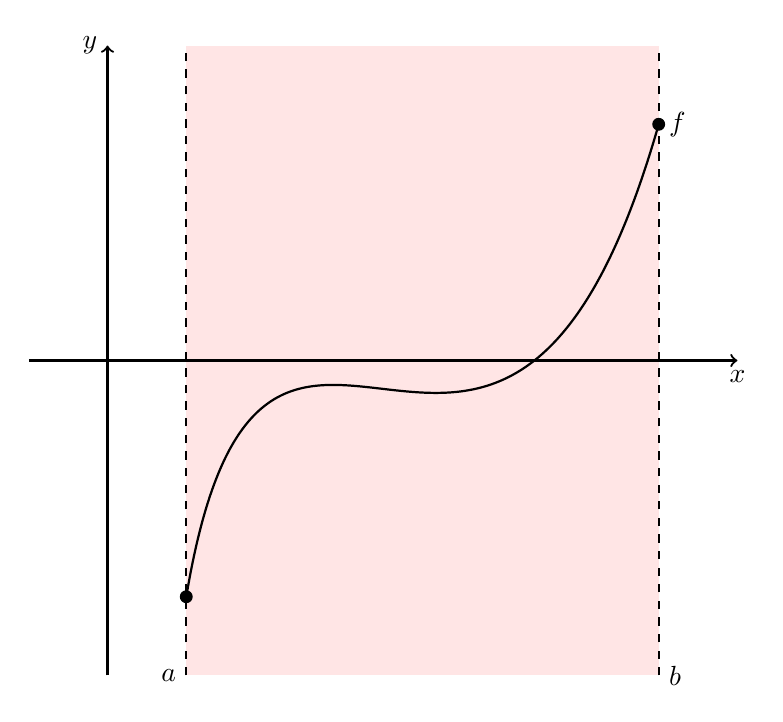
\begin{tikzpicture}
		\fill[red!10] (1,-4) rectangle (7,4);
		\draw[thick, ->] (-1,0) -- (8,0)node[pos=1, below]{$x$};
		\draw[thick, ->] (0,-4) -- (0,4)node[pos=1, left]{$y$};
		\draw[thick] (1,-3) .. controls (2,3) and (5,-4) .. (7,3) node[right]{$f$};
		\node[circle, inner sep=1.5pt, fill=black, draw=black] (a) at (1,-3){};
		\node[circle, inner sep=1.5pt, fill=black, draw=black] (b) at (7,3){};
		\draw[dashed, thick] (1,-4) -- (1,4) node[pos=0,left]{$a$};
		\draw[dashed, thick] (7,-4) -- (7,4) node[pos=0,right]{$b$};
		\end{tikzpicture}
	\end{frame}
	\begin{frame}
		\centering
		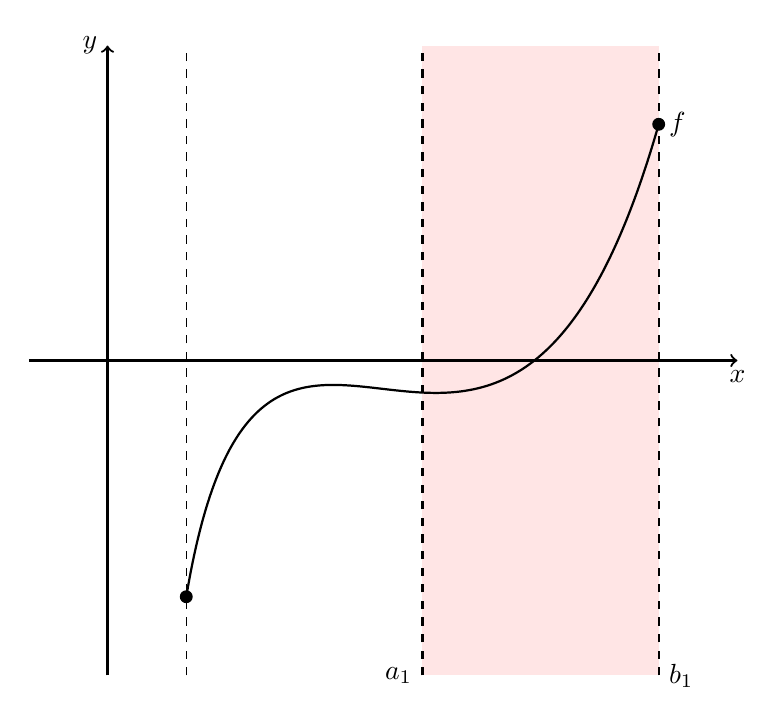
\begin{tikzpicture}
		\fill[red!10] (4,-4) rectangle (7,4);
		\draw[thick, ->] (-1,0) -- (8,0)node[pos=1, below]{$x$};
		\draw[thick, ->] (0,-4) -- (0,4)node[pos=1, left]{$y$};
		\draw[thick] (1,-3) .. controls (2,3) and (5,-4) .. (7,3) node[right]{$f$};
		\node[circle, inner sep=1.5pt, fill=black, draw=black] (a) at (1,-3){};
		\node[circle, inner sep=1.5pt, fill=black, draw=black] (b) at (7,3){};
		\draw[dashed] (1,-4) -- (1,4);
		\draw[dashed, thick] (4,-4) -- (4,4) node[pos=0,left]{$a_1$};
		\draw[dashed, thick] (7,-4) -- (7,4) node[pos=0,right]{$b_1$};
		\end{tikzpicture}
	\end{frame}
	\begin{frame}
		\centering
		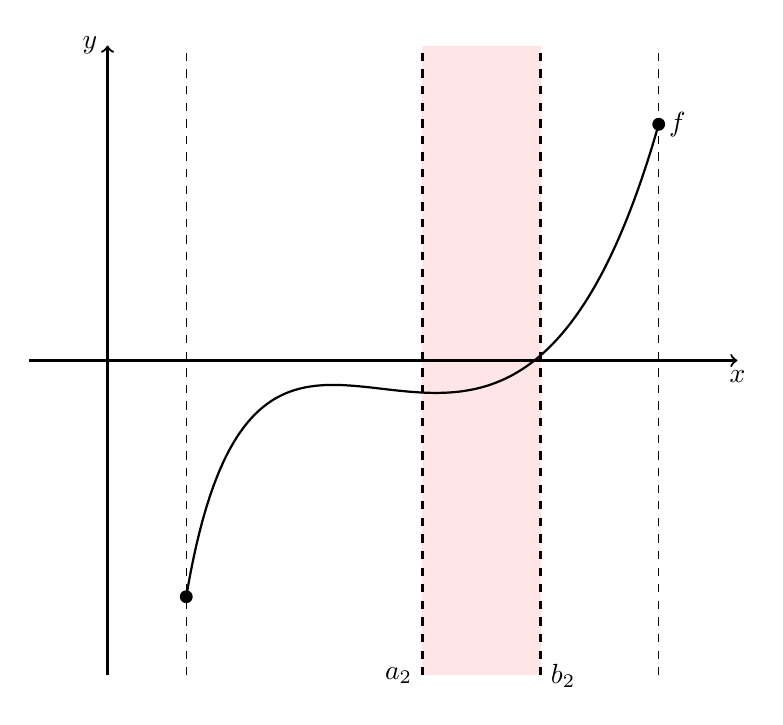
\begin{tikzpicture}
		\fill[red!10] (4,-4) rectangle (5.5,4);
		\draw[thick, ->] (-1,0) -- (8,0)node[pos=1, below]{$x$};
		\draw[thick, ->] (0,-4) -- (0,4)node[pos=1, left]{$y$};
		\draw[thick] (1,-3) .. controls (2,3) and (5,-4) .. (7,3) node[right]{$f$};
		\node[circle, inner sep=1.5pt, fill=black, draw=black] (a) at (1,-3){};
		\node[circle, inner sep=1.5pt, fill=black, draw=black] (b) at (7,3){};
		\draw[dashed] (1,-4) -- (1,4);
		\draw[dashed, thick] (4,-4) -- (4,4) node[pos=0,left]{$a_2$};
		\draw[dashed, thick] (5.5,-4) -- (5.5,4) node[pos=0,right]{$b_2$};
		\draw[dashed] (7,-4) -- (7,4);
		\end{tikzpicture}
	\end{frame}
	\begin{frame}
		\centering
		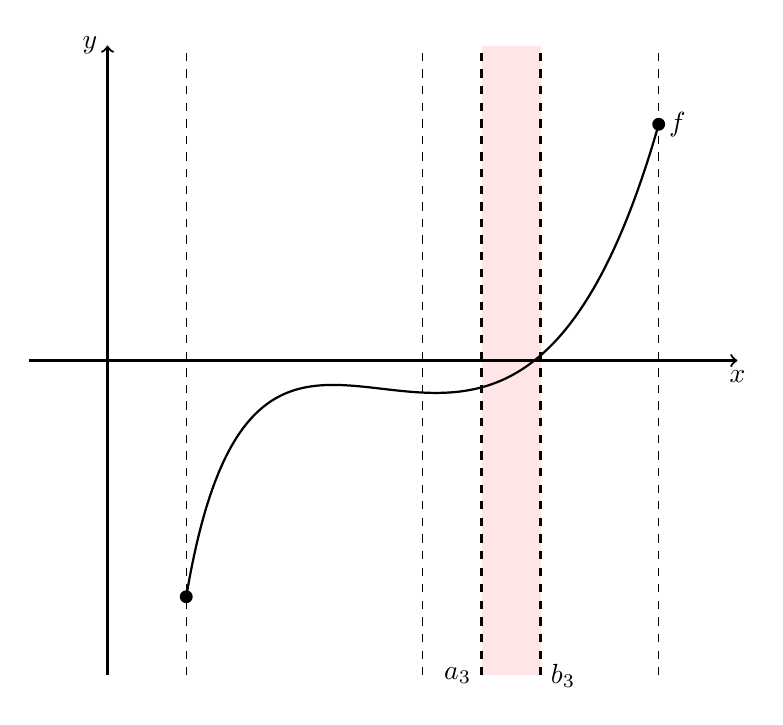
\begin{tikzpicture}
		\fill[red!10] (4.75,-4) rectangle (5.5,4);
		\draw[thick, ->] (-1,0) -- (8,0)node[pos=1, below]{$x$};
		\draw[thick, ->] (0,-4) -- (0,4)node[pos=1, left]{$y$};
		\draw[thick] (1,-3) .. controls (2,3) and (5,-4) .. (7,3) node[right]{$f$};
		\node[circle, inner sep=1.5pt, fill=black, draw=black] (a) at (1,-3){};
		\node[circle, inner sep=1.5pt, fill=black, draw=black] (b) at (7,3){};
		\draw[dashed] (1,-4) -- (1,4);
		\draw[dashed] (4,-4) -- (4,4);
		\draw[dashed, thick] (4.75,-4) -- (4.75,4) node[pos=0,left]{$a_3$};
		\draw[dashed, thick] (5.5,-4) -- (5.5,4) node[pos=0,right]{$b_3$};
		\draw[dashed] (7,-4) -- (7,4);
		\end{tikzpicture}
	\end{frame}
	\begin{frame}
		\centering
		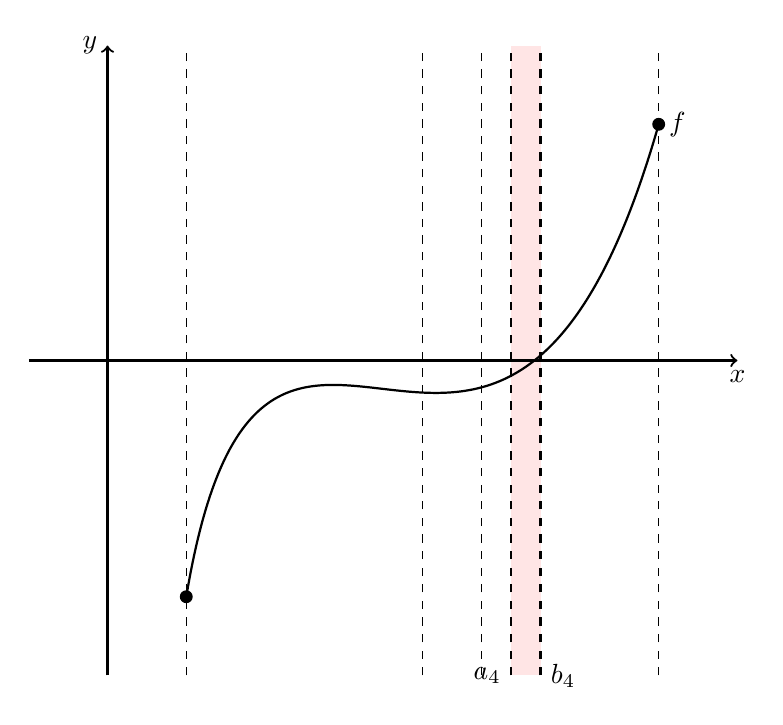
\begin{tikzpicture}
		\fill[red!10] (5.125,-4) rectangle (5.5,4);
		\draw[thick, ->] (-1,0) -- (8,0)node[pos=1, below]{$x$};
		\draw[thick, ->] (0,-4) -- (0,4)node[pos=1, left]{$y$};
		\draw[thick] (1,-3) .. controls (2,3) and (5,-4) .. (7,3) node[right]{$f$};
		\node[circle, inner sep=1.5pt, fill=black, draw=black] (a) at (1,-3){};
		\node[circle, inner sep=1.5pt, fill=black, draw=black] (b) at (7,3){};
		\draw[dashed] (1,-4) -- (1,4);
		\draw[dashed] (4,-4) -- (4,4);
		\draw[dashed] (4.75,-4) -- (4.75,4);
		\draw[dashed, thick] (5.125,-4) -- (5.125,4) node[pos=0,left]{$a_4$};
		\draw[dashed, thick] (5.5,-4) -- (5.5,4) node[pos=0,right]{$b_4$};
		\draw[dashed] (7,-4) -- (7,4);
		\end{tikzpicture}
	\end{frame}
\end{document}